\chapter{Mission}
  \section{Projet}

      Ce rapport de stage constitue un livrable dans le cadre du projet
      ImpRo\footnotemark pour {\it Implementatbility and Robustness of Timed
        Systems}. Ce projet est financé par l'Agence Nationale de la Recherche
      dans le cadre du Programme Blanc. Il s’interesse aux problèmes liés aux
      implémentations des modèles formels des systèmes embarqués communicants.
      \footnotetext{\url{http ://anr-impro.irccyn.ec-nantes.fr}}

      ~
    
      Les différentes entitées universitaires collaborant à ce projet sont
      l'IRCCyN (Nantes), l'IRISA (Rennes), le LIP6, le LSV, le LIAFA (Paris) et
      le LIF (Marseille). Son coordinateur est Didier Lime de l'équipe Systèmes
      Temps Reél de l'IRCCyN.

      ~
      
      Ce projet adresse les problèmes liés aux mises en \oe uvre pratiques des
      modélisations formelles des systèmes embarqués communicants. Ces modèles
      abstraient beaucoup d’aspects complexes ou de limitations de leur
      environnement d’exécution. La modélisation du temps, en particulier, est
      habituellement idéale, avec des horloges infiniment précises, des tests ou
      des changements de mode instantanés. L’objectif de ce projet est d’étudier
      dans quelle mesure les implémentations de ces modèles préservent leurs
      propriétés.

      ~
    
      La robustesse d’un modèle caractérise l’amplitude de la différence
      existant entre ce modèle et une mise en \oe uvre qui en est faite. Cette
      difference réside, pour une part, dans l’écart entre la modèlisation d’un
      système et son implementation, pour une autre part, dans l’écart entre la
      modélisation de l’environement du système et l’environement réellement
      constaté. Si un écart faible ne permet pas de préserver les propriétés
      constatées sur le modèle alors celui-ci est considéré comme peu robuste.
      L'un des objectifs du projet est de mesurer et éventuellement réduire la
      distance qui existe entre un modèle d'un système et sa réalisation.

      ~
    
      Plusieurs approches d'analyse de robustesse des modèles temporisés ont été
      développées dans le cadre de ce projet. Dans ce rapport nous nous
      concentrons sur deux d'entre elles. La première approche s'appuie sur la
      réduction des automates temporisés, la seconde sur la synthèse de
      paramètres temporels.

      ~

      Afin de
      mettre en évidence les résultats théoriques issus de ce projet il a été
      proposé de réaliser un démonstrateur. Celui-ci est un système réel qui peut
      être modélisé et analysé à l'aide des outils mathématiques étudiés dans le
      projet. Une spécification du démontrateur a été réalisée \cite{bechennec12}.

    \subsection{Spécification}

      \begin{figure}
        \centering
        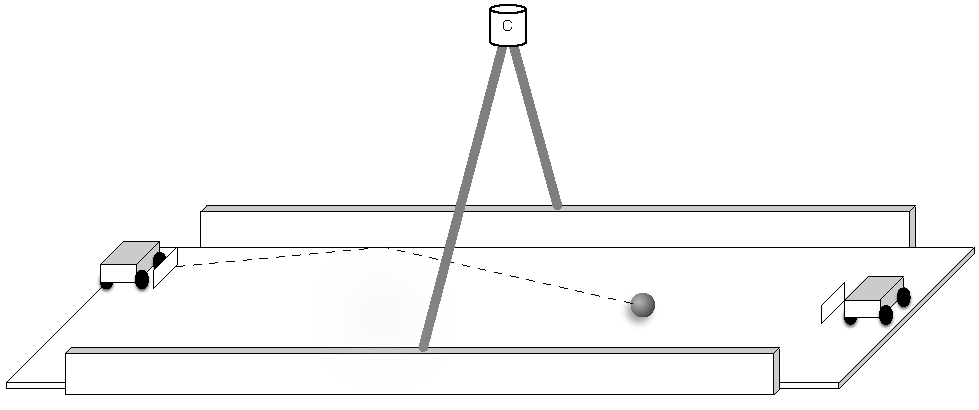
\includegraphics[width=0.8\textwidth]{./img/spec-demo1.pdf}
        \caption{Schéma de la spécification, vue isométrique}
        \label{fig:spec-demo1}
      \end{figure}

      \begin{figure}
        \centering
        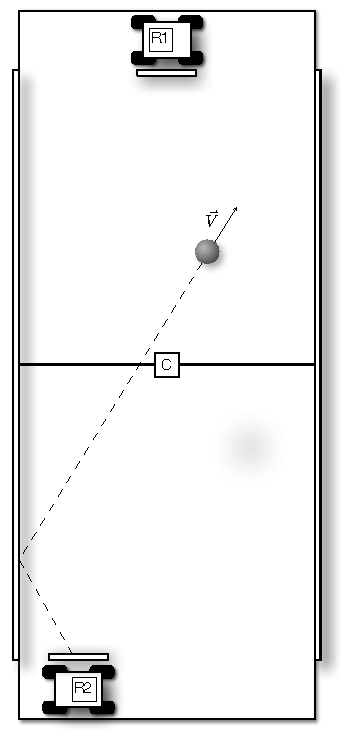
\includegraphics[angle=270, width=0.8\textwidth]{./img/spec-demo2.pdf}
        \caption{Schéma de la spécification, vue du dessus}
        \label{fig:spec-demo2}
      \end{figure}

      Le démonstrateur est un système de deux robots qui jouent à un jeu inspiré
      du {\it air kockey}. Dans ce jeu, chaque joueur cherche à faire sortir la
      balle du terrain par le côté du joueur adverse. Le terrain est représenté
      vu du dessus sur la figure \ref{fig:spec-demo1} et en perspective
      isométrique sur la figure \ref{fig:spec-demo2}. Le terrain est
      rectangulaire. Les longueurs sont équipées de rebords sur lesquels la
      balle vient rebondir. Les robots sont équipés d'un dispositif permettant
      de récupérer et de frapper la balle ainsi que de roues non
      directrices. Ils se déplacent dans le sens de la largeur du terrain, sur
      des rigoles.

      ~
    
      Les robots sont réalisés à l'aide du kit robotique Lego Mindstorms NXT. Le
      système d'exploitation temps réel Trampoline est utilisé pour exploiter
      les microcontrôleurs qui équipent ces kits. Ce système d'exploitation est
      un logiciel libre dont le développement est principalement assuré par
      l'équipe Systèmes Temps Réel de l'IRCCyN.

      ~
    
      Le logiciel de pilotage des robots est un logiciel temps réel. Des
      contraintes temps réel sont ainsi associées aux fonctions de pilotage des
      organes du robot (moteur qui entraîne les roues, moteurs de manipulation
      de la raquette), et aux fonctions de planification des déplacements
      (récupération de la trajectoire de la balle, positionnement en regard de
      la balle). Le système d'exploitation Trampoline offre les services
      nécessaires à la garantie de ces contraintes.
  
      ~
    
      Pour déterminer la position à atteindre pour pouvoir frapper la balle, les
      robots interrogent une station centrale qui fournit la position et
      l'accélération de la balle. Cette information est capturée à l'aide d'une
      caméra située au-dessus du terrain.

      \subsubsection{Modifications des spécifications}

        Par contrainte technique, certains éléments de cette spécification
        initiale ont été ajustés afin de garantir la faisabilité du
        démonstrateur. En effet, des essais préalables ont montré que les temps
        de latence des communications de la station centrale vers les robots
        cumulés aux temps de traitements sur la station centrale étaient trop
        important pour permettre la réalisation du démonstrateur.

        ~
    
        L'implémentation actuelle n'inclus pus de station centrale. Son rôle de
        détection de la balle a été remplacée par une caméra embarquée pouvant
        réaliser des traitements d'images simples. Cette caméra est associée à
        un Arduino Uno réalisant la communication avec le robot Lego via un bus
        I2C.

        ~
        
        La mise en \oe uvre de cette modification de la spéficiation du
        démonstrateur a donné lieu à un stage réalisé par Benjamin Sientzoff
        s'étant déroulé de Juin à Juillet 2014.

  \section{Besoin}

    Le travail attendu est la réalisation d'une étude de cas non-triviale sur
    la robustesse des modèles temporisés s'appuyant sur le démonstrateur issu
    du projet ImpRo. Ce travail s'articule en plusieurs volets : la
    modélisation du démonstrateur, l'implémentation du modèle réalisé et des
    vérifications formelles et pratique des propriétés du modèle.

    \subsection{Modélisation}

      Deux types de modélisations sont attendues. La première modélisation
      attendue est une modélisation architecturale du démonstrateur. Elle décrit
      l'architecture matérielle et logicielle du démonstrateur. Cette
      modélisation a pour principal objectif d'être un support de
      documentation sur l'arichitecture du démonstrateur. Elle doit permettre
      aux personnes travaillant sur d'autre aspect dans le cadre du projet
      Impro ou dans le cadre d'autres projets aux thématiques avoisinantes
      d'appréhender le fonctionnement du démonstrateur de manière simple.

      Un des rôles de cette modélisation est en conséquence d'introduire des
      noms qui pourront être retrouvés dans la seconde modélisation. Ces noms
      permettront de faire le lien entre les deux modélisations.

      ~
  
      La seconde modélisation attendue est une modèlisation comportementale du
      démontrateur. Elle définit le comportement de celui-ci. Ce sont les
      modèles issus de cette modélisation qui serviront de support aux
      différentes analyses et vérifications qui sont attendues. Un des rôles
      de cette modélisation est également de servir de support à
      l'implémentation des robots du démonstrateur.

    \subsection{Implémentation}

      Suite à certaines contraintes propre à l'équipe Système Temps Réel,
      l'implémentation matérielle du démonstrateur n'a pu être complétement
      réalisée avant le début de mon stage. Ce démonstrateur a vocation à être
      réutiliser dans le cadre d'autres projets de recherche. Il est donc
      attendu un travail soigné et documenté qui puisse être facilement
      réutiliser par d'autres personnes, stagiaires comme
      enseignants-chercheurs.

      ~

      Il m'est donc demandé de
      travailler à compléter ainsi qu'à modifier l'implémentation matérielle
      du démonstrateur. Celle-ci doit integrer un permier moteur pour le
      déplacement latéral, un second moteur pour la manipulation de la
      raquette permettant le tir, une caméra permettant de suivre la balle à
      distance, des capteurs de proximité permettant de repérer la balle à
      proximité et un capteur de distance permettant de définir le
      positionnement latéral du robot.

      ~
  
      L'implémentation logicielle doit assurer des propriétés temps réel. Elle
      sera donc réalisée grâce à un jeu de tâches qui sera ordonnancé par
      un système d'exploitation temps réel. Ces tâches doivent réalisées les
      fonctions liées à l'implémentation matérielle. C'est à dire commander le
      déplacement latéral du robot en fonction de la position de la balle et
      celle du robot ainsi qu'actionner la raquette afin de tirer dans la balle
      lorsque celle-ci se trouve à proximité.

    \subsection{Vérification}

      Les vérifications qui seront réalisées constitueront une mise en \oe
      uvre des résultats de recherche issu du projet Impro. Cette mise en \oe
      uvre prendra la forme de vérifications formelles sur des modèles
      temporisés. Les résultats de ces vérifications nous donnerons un
      indicateur quand à la robustesse des modèles considérés.

      ~
      
      Les propriétés que l'on souhaite vérifier sont en rapport avec la notion
      de robustesse des modèles. Ici, on souhaite montrer que telle ou telle
      sous-partie du modèle du système est robuste ou non-robuste. De même, on
      souhaite montrer que sous certaines contraintes liées à l'implémentation
      du modèle le système est faisable ou non en regard à un comportement
      attendu du démonstrateur. 

      Une fois les résultats théoriques sur la robustesse du démonstrateur
      obtenus, ceux-ci pourront être analysé et comparer aux constatations
      concrètes qui peuvent être fais sur le fonctionnement du démonstrateur.

